% ------------------------------------------------------------------------
% ------------------------------------------------------------------------
% ICMC: Modelo de Trabalho Acadêmico (tese de doutorado, dissertação de
% mestrado e trabalhos monográficos em geral) em conformidade com 
% ABNT NBR 14724:2011: Informação e documentação - Trabalhos acadêmicos -
% Apresentação
% ------------------------------------------------------------------------
% ------------------------------------------------------------------------

% Opções: 
%   Qualificação         = qualificacao 
%   Curso                = doutorado/mestrado
%   Situação do trabalho = pre-defesa/pos-defesa (exceto para qualificação)
% -- opções do pacote babel --
% Idioma padrão = brazil
	%french,	    	% idioma adicional para hifenização
	%spanish,			% idioma adicional para hifenização
	%english,			% idioma adicional para hifenização
	%brazil				% o último idioma é o principal do documento
\documentclass[brazil]{packages/icmc}

% Tag <hr> como comando \hr
\newcommand\hr{\par\vspace{-.5\ht\strutbox}\noindent\hrulefill\par}

% Comando simples para exibir comandos Latex no texto
\newcommand{\comando}[1]{\textbf{$\backslash$#1}}
% métodos em java
\newcommand{\method}[1]{\textit{#1}}

% ---
% Pacotes Opcionais
% ---
\usepackage{rotating}           % Usado para rotacionar o texto
\usepackage[all,knot,arc,import,poly]{xy}   % Pacote para desenhos gráficos
% Este pacote pode conflitar com outros pacotes gráficos como o ``pictex''
% Então é necessário usar apenas um dos pacotes conflitantes


% ---
% Informações de dados para CAPA e FOLHA DE ROSTO
% ---
\titulo{Algoritmo evolutivo para treinar um sistema inteligente para jogos de disputa}
\autor[Bastiani, L. G.]{Leonardo Guarnieri de Bastiani}
\orientador[Orientador:]{Prof. Dr.}{Eduardo do Valle Simões}
%\coorientador{Prof. Dr.}{Fulano de tal}
\curso{Engenharia de Computação}
\area{Computação Bioinspirada} % Área de concentração do trabalho
\data{08}{11}{2018} % Data do depósito
% ---


% ---
% RESUMOS
% ---

% Resumo em português
% conter no máximo 500 palavras
\newcommand{\fitness}{\textit{fitness}\xspace}
\textoresumo{
    Este trabalho trata do desenvolvimento de um algoritmo bioinspirado capaz de treinar um sistema inteligente para aprender a emular comportamento em jogos de disputa. Nos jogos do contexto deste algoritmo, há decisões a serem tomadas por dois jogadores, dependendo da situação de cada jogada. Para isso, o algoritmo evolutivo ajusta os parâmetros que são usados na tomada de decisão. Para o algoritmo, a função \fitness é a comparação dos resultados apresentados pelas soluções que forem sendo geradas para selecionar as mais adequadas para gerar novas alternativas de controladores.
    }{Computação bioinspirada, algoritmo evolutivo, aprendizado de máquina, gamificação}

% ---
% resumo em inglês
% ---
\textoresumo[english]{
    This project is about a development of a bioinspired algorithm capable of training an intelligent system to learn how to emulate behavior in dispute games. In the games in the context of this algorithm, there are decisions to be made by two players, depending on the situation of each move. The evolutionary algorithm adjusts the parameters that are used in the decision making. The \fitness function is the comparison of the results presented by the solutions that are generated to select the most suitable ones to generate new alternatives of controllers.
    }{Bio-inspired computation, evolutionary algorithm, machine learning, gamification}
    
% ---
% Configurações de aparência do PDF final
% ---
% alterando o aspecto da cor azul
\definecolor{blue}{RGB}{41,5,195}

% informações do PDF
\makeatletter
\hypersetup{
     	pagebackref=true,
		pdftitle={\@title}, 
		pdfauthor={\@author},
    	pdfsubject={\imprimirpreambulo},
	    pdfcreator={LaTeX with abnTeX2/ICMC-USP},
		pdfkeywords={\palavraschave}, 
		colorlinks=true,       		% false: boxed links; true: colored links
    	linkcolor=blue,          	% color of internal links
    	citecolor=blue,        		% color of links to bibliography
    	filecolor=magenta,      	% color of file links
		urlcolor=blue,
		bookmarksdepth=4
}
\makeatother
% --- 

% ----------------------------------------------------------
% ELEMENTOS PRÉ-TEXTUAIS
% ----------------------------------------------------------

% Inserir a ficha catalográfica
%\incluifichacatalografica[tex/fichaCatalografica.pdf]
\incluifichacatalografica


% Inserir folha de aprovação
%
% Isto é um exemplo de Folha de aprovação, elemento obrigatório da NBR
% 14724/2011 (seção 4.2.1.3). Você pode utilizar este modelo até a aprovação
% do trabalho. Após isso, substitua todo o conteúdo deste arquivo por uma
% imagem da página assinada pela banca com o comando abaixo:
%
% \includepdf{folhadeaprovacao_final.pdf}
%
\begin{folhadeaprovacao}

  \begin{center}
    {\ABNTEXchapterfont\large\imprimirautor}

    \vspace*{\fill}\vspace*{\fill}
    {\ABNTEXchapterfont\bfseries\Large\imprimirtitulo}
    \vspace*{\fill}
    
    \hspace{.45\textwidth}
    \begin{minipage}{.5\textwidth}
        \imprimirpreambulo
    \end{minipage}%
    \vspace*{\fill}
   \end{center}
    
   Trabalho aprovado. \imprimirlocal, 24 de novembro de 2012:

   \assinatura{\textbf{\imprimirorientador} \\ Orientador} 
   \assinatura{\textbf{Professor} \\ Convidado 1}
   \assinatura{\textbf{Professor} \\ Convidado 2}
   %\assinatura{\textbf{Professor} \\ Convidado 3}
   %\assinatura{\textbf{Professor} \\ Convidado 4}
      
   \begin{center}
    \vspace*{0.5cm}
    {\large\imprimirlocal}
    \par
    {\large\imprimirdata}
    \vspace*{1cm}
  \end{center}
  
\end{folhadeaprovacao}
% ---

% DEDICATÓRIA / AGRADECIMENTO / EPÍGRAFE
\textodedicatoria*{tex/pre-textual/dedicatoria}
\textoagradecimentos*{tex/pre-textual/agradecimentos}
\textoepigrafe*{tex/pre-textual/epigrafe}

% Inclui a lista de figuras
\incluilistadefiguras

% Inclui a lista de tabelas
\incluilistadetabelas

% Inclui a lista de quadros
\incluilistadequadros

% Inclui a lista de algoritmos
\incluilistadealgoritmos

% Inclui a lista de códigos
\incluilistadecodigos

% Inclui a lista de siglas e abreviaturas
\incluilistadesiglas

% Inclui a lista de símbolos
\incluilistadesimbolos

% ----
% Início do documento
% ----
\begin{document}

% ----------------------------------------------------------
% ELEMENTOS TEXTUAIS
% ----------------------------------------------------------
\textual

\chapter{Introdução}
\label{chapter:introducao}
\section{Motivação e Contextualização}

\newcommand\SE{\sigla{SE}{Sistema Evolutivo}\xspace}

Este trabalho relata a criação de uma biblioteca que aplica os conceitos de Computação Bioinspirada e sua aplicação em um sistema desconhecido com entradas e saídas bem definidas. O uso de algoritmos evolutivos é um contraste de algoritmos determinísticos  e incorporam outro viés de solução por um \SE\cite{Layzell1999} para ajustar continuamente os parâmetros de controlador às variações na configuração do ambiente de trabalho.

A área de pesquisa conhecida como Computação Bioinspirada procura encontrar soluções elegantes e eficientes que resolvem problemas grandes que poderiam demandar tempo computacional incompatível com a necessidade de resposta através de técnicas tradicionais. O comportamento social de formigas e abelhas, estratégia de caça de predadores ou o ciclo de atividade e hibernação de ursos são modelos e inspirações para essa área, estes exemplos ilustram soluções de problemas que podem incluir otimização, orientação e reconhecimento de padrões, tudo isso sendo obtido através de um processo evolutivo.\footnote{Simões, E. D. V. (2000). Indelevelmente Of An Embedded Evolutionary Controller To Enable Collision-Free Navigation Of A Population Of Autonomous Robots. University of Kent at Canterbury, Inglaterra p. 289}

A técnica estudada neste trabalho denomina-se Computação Evolutiva da calsse de técnicas conhecida como Computação Biológica ou Biocomputação que se inspira em princípios biológicos para projetar o algoritmo computacional, mais especificamente no comportamento social de organismos.

Um algoritmo evolutivo é capaz de caminhar a solução de um problema através da comparação de uma função \fitness que é uma função de comparação entre duas soluções. Por tanto, nesse trabalho, a ferramenta desenvolvida tem sua função \fitness como a comparação entre duas entidades que competem, o vencedor é aquele com uma melhor função \fitness. Foi estudada uma aplicação desse algoritmo com a comparação entre um sistema qualquer com entradas e respostas de modo a prever as possíveis respostas do sistema.

\section{Objetivos}

Este trabalho visa desenvolver uma biblioteca de algoritmo evolutivo que se enquadra em situações onde pode-se comparar duas soluções por meio de disputas capaz de se adaptar às alterações de cada cenário e estudar sua aplicação em um sistema com entradas e saídas bem definidas de modo a prever novas saídas.

A biblioteca implementa os conceitos de Indivíduo, que é um dos participantes de uma disputa, e de Gene, que é um dos fatores que determinará como um indivíduo responde a uma entrada. Nos estudos da utilização dessa ferramenta, foram feitos sistemas com saídas que seguem uma determinada lógica e os resultados foram comparados com um sistema que gera saídas aleatoriamente.

\section{Organização}

Este documento relata os métodos desenvolvidos e aplicados para a construção do algoritmo, além de citar fontes que comprovam a eficácia e estudos com aplicações do algoritmo que o validam.

O código-fonte produzido para essa aplicação está disponibilizado\footnote{\url{https://github.com/leobastiani/AE}} e uso da biblioteca para novas ferramentas que podem ser modeladas nos casos propostos, isto é, que são capazes de realizar disputas entre dois, gerando um melhor vencedor e um perdedor.


\chapter{Métodos, Técnicas e Tecnologias Utilizadas}
\label{chapter:metodos}
\section{Revisão Bibliográfica} \label{secao:rev_bib}

A inspiração do paradigma da Computação Evolutiva vem da evolução natural formalizada por Darwin \cite{Ridley1996}. Algoritmos embebidos desta tese possuem passos genéricos capazes de resolver um grande número de problemas práticos, e possuem características como auto-organização e comportamento adaptativo \cite{Goldberg1988}, portanto são capazes de tratar problemas computacionalmente complexos com uma ferramenta de propósito geral. Por outro lado, esses algoritmos não garantem a obtenção de uma solução ótima \cite{Zuben2000} por poder convergir para soluções localmente ótimas.

A linguagem de programação Java foi escolhida para a criação da ferramenta, os motivos para essa escolha foram:

\newcommand{\JVM}{\sigla{JVM}{Java Virtual Machine}\xspace}

\begin{itemize}
    \item Multiplataforma: Java é uma linguagem capaz de ser executada em qualquer sistema que possua uma \JVM, sua execução e desenvolvimento independe do sistema, permitindo que a aplicação desenvolvida não sofra essa restrição.
    \item Desempenho: entre as linguagens de programação que são interpretadas, Java possui um desempenho melhor por ser compilada e interpretada, gerando um código intermediário que é executado pela \JVM.
    \item Facilidade e didática: Java é uma linguagem que permite certas comodidades ao programador com um bom balanço de desempenho, como a ferramenta desenvolvida foi utilizada para estudos e é de uso genérico, as facilidades fornecidas pela linguagem são importante para agilizar e pela validação do trabalho.
    \item Modelagem: a modelagem de classes fornecida por Java ajudam no entendimento e no reuso da biblioteca desenvolvida.
\end{itemize}

Nesse projeto há uma contextualização do problema nos seguintes moldes:

\begin{itemize}
    \item Indivíduo: um indivíduo é a representação de um jogador que possui uma pontuação provida da função \fitness de acordo com as respostas produzidas por esse jogador.
    \item Gene: um gene é uma entidade capaz de provocar uma resposta. Para cada tipo de respostas há um grupo de genes. As entradas de um sistema são capazes de excitar o gene e o gene mais excitado responde pelo indivíduo.
    \item Disputa: é uma função entre dois indivíduos que gera um vencedor e um perdedor com base na função \fitness. Uma disputa deve necessariamente retornar o quão melhor um indivíduo foi em relação a outro.
\end{itemize}

Por tanto, o indivíduo que possui os melhores genes terá uma função \fitness melhor e ganhará mais disputas.

\section{Algoritmos evolutivos}
Os algoritmos evolutivos podem ser resumidos em um roteiro básico de procedimentos \cite{Todd1997} que são adaptados de acordo com o contexto do problema a ser solucionado \cite{Werger1999} \cite{Mitchell1995}. Um algoritmo evolutivo é usualmente composto por:

\newcommand{\crossover}{\textit{crossover}\xspace}

\begin{itemize}
    \item Representação de genes dos indivíduos: Biologicamente, cada gene representa uma característica do indivíduo, e o cromossomo, que é o conjunto de genes de um indivíduo, representa o indivíduo. Computacionalmente, o cromossomo representa um candidato à solução do problema e o gene representa uma função para obtenção de uma resposta.
    \item Função \fitness (ou de adaptação): indica, para cada indivíduo, o valor de aptidão, mostrando a aproximação da solução proposta pelo indivíduo em relação à solução procurada.
    \item Função de reprodução: Determina novos indivíduos que representarão a próxima geração da população do algoritmo herdando características que são encontradas nos indivíduos com uma maior função \fitness (ou mais aptos), propagando seus genes. O \crossover e mutações ocorrem na função de reprodução, de modo análogo ao biológico.
\end{itemize}

Em um algoritmo evolutivo, a população inicial é constituída por indivíduos com genes aleatórios, ou seja, o início do algoritmo parte de uma solução aleatória e a cada geração, o valor de \fitness ou adequação é calculado em cada indivíduo. A função de reprodução gera novos indivíduos e as características positivas de cada indivíduo podem ser propagadas para a nova geração, assim a solução caminha para uma resposta adequada. O fluxograma na Figura \ref{figura:fluxograma_ae} representa estas etapas.

\begin{figure}[htb]
    \caption{Fluxograma de uma implementação típica de um algoritmo evolutivo.}
    \label{figura:fluxograma_ae}
    \centering
    %scale=0.8
    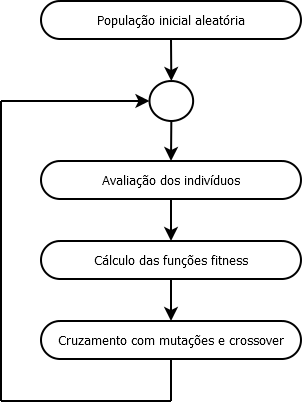
\includegraphics[scale=1]{images/dia/fluxograma-ae}
    \fautor
\end{figure}

\chapter{Desenvolvimento}
\label{chapter:desenvolvimento}
\section{O Problema}

O projeto consiste do desenvolvimento de uma biblioteca de algoritmo evolutivo genérica para solucionar problemas com gamificação de disputas, ou seja, encontrar soluções que possam ser comparadas através de uma disputa entre dois jogadores, gerando um vencedor e um perdedor necessariamente. Bem como estudar as aplicações desse algoritmo em um sistema com entradas e saídas bem definidas, de modo que a solução não esteja implícita em nenhuma das entradas e saídas, mas que o algoritmo possa evoluir livremente para encontrar o melhor rearranjo dos genes até produzir respostas idênticas as oferecidas pelo sistema.

\section{Biblioteca de Algoritmos Evolutivos}

Foi feita uma biblioteca para uso de algoritmos evolutivos em Java que emprega os conceitos de Indivíduos e Genes. Para aplicações diferentes das estudadas nesse documento, a biblioteca ainda pode ser usada em qualquer \SE, pois pode ser estendida e rearranjada para qualquer aplicação dentro desse conceito. As classes e métodos implementadas pela biblioteca estão descritas a seguir.

\subsection{Classe AE}

Esta classe é responsável por englobar as funções referentes ao algoritmo evolutivo em si, ou seja, ela organiza e remaneja os indivíduos, realiza confrontos, compara soluções, seleciona os melhores e recombina os indivíduos de modo que as melhores soluções propaguem suas características.

As disputas realizadas pelos indivíduos seguem um sistema de torneio mata-mata\footnote{\url{https://pt.wikipedia.org/wiki/Competições_eliminatórias}}, que por padrão possui 16 participantes, no qual o primeiro e segundo colocados cruzam suas características genéticas com os indivíduos que não foram enfrentados por eles.

\begin{figure}[htb]
    \caption{Torneio realizado pela classe AE. A ilustração demonstra um caso em que o campeão do torneio veio dos indivíduos de 0 a 7 e o vice-campeão veio dos indivíduos de 8 a 15.}
    \label{figura:funcao_playAll}
    \centering
    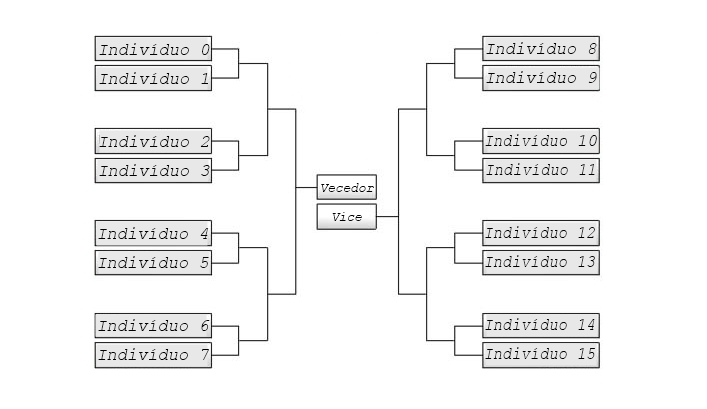
\includegraphics[scale=0.8]{images/ps/mata-mata}
    \fautor
\end{figure}

Neste torneio, há dois grupos, o grupo da esquerda composto pelos indivíduos de 0 a 7 e o grupo da direita composto pelos indivíduos de 8 a 15. O campeão do torneio transmite os genes para o grupo em que não obteve confrontos, com exceção do vice-campeão, e o mesmo ocorre para o vice-campeão.

A Figura \ref{figura:funcao_playAll} demonstra como funciona esse torneio e a propagação das características dos melhores colocados, exemplificando que o indivíduo campeão estava entre os indivíduos de 0 a 7 e o vice-campeão estava entre os indivíduos de 8 a 15, sendo assim, o campeão transmite suas características genéticas para os indivíduos de 8 a 15, com exceção do vice-campeão, e vice-versa.

A classe AE possui outras funções implementadas que são de uso diverso e serão discutidas em outra subseção.

\subsection{Classe Eq}

\newcommand{\var}[1]{\textit{#1}}

A classe Eq representa uma equação e possui uma função como representa a equação \ref{eq:eq}. Onde as variáveis \var{factor} e \var{sum} correspondem a variáveis internas da classe e constituem parte de um gene.

\begin{equation}
    \label{eq:eq}
    f(x)=\mathrm{factor}*x + \mathrm{sum}
\end{equation}

\subsection{Classe Indivíduo}

A classe indivíduo representa um indivíduo capaz de gerar uma solução para o sistema. A função \fitness de cada indivíduo é responsável por informar o quão boa é a solução deste indivíduo. Se um indivíduo ganha mais confrontos do que outro, sua função \fitness será maior.

Na biblioteca, o indivíduo possui o método \method{play} que recebe outro indivíduo como parâmetro. O usuário escolhe como confrontar os dois indivíduos retornando 0 se o vencedor for indivíduo que chama o método, ou 1, se o vencedor for o indivíduo referenciado no parâmetro. Nesta função não é possível retornar uma informação para os casos de empate. Como este projeto foca uma disputa entre dois indivíduos, o método \method{play} pode confrontar esses dois indivíduos $N$ vezes e basear sua função \fitness na quantidade de partidas vencidas, além de retornar o indivíduo que mais venceu partidas como vitorioso.

\subsection{Classe Gene}

Cada indivíduo pode possuir uma determinada quantidade de genes que são capazes de gerar uma resposta. O gene pode ser excitado de alguma forma pelo sistema e possui um valor de estado que pode aumentar de acordo com a operação operação de consumir um estado. Portanto um gene possui duas funções que envolvem a variável \var{estado}:

\begin{itemize}
    \item \method{Consumir}: O método de \method{consumir} altera a variável \var{estado} do gene conforme a equação \ref{eq:gene_consumir} onde $x$ é o valor da entrada, $i$ é a posição da entrada no ventor de entradas de um sistema, ou seja, se um sistema possui entradas com vetor de tamanho $N$, $i$ terá valores de 0 até $N-1$, $E$ e $I$ são funções descritas em \ref{eq:eq}.
    \begin{equation}
        \label{eq:gene_consumir}
        \mathrm{Estado} \leftarrow \mathrm{Estado} +  E(x) * I_i(i)
    \end{equation}
    \item \method{Reset}: O método de \method{reset} devolve o \var{estado} do gene para um estado inicial. A classe Gene possui as variáveis internas \var{estado}, \var{estadoInicial}, \var{limiteSup} e \var{limiteInf}. A função de \method{reset} está descrita no algoritmo \ref{algoritmo:gene_reset}.
\end{itemize}

\begin{algoritmo}
\caption{Algoritmo de reinicio de gene.}
\label{algoritmo:gene_reset}
    \If(\tcp*[f]{Se o estado do gene está fora dos limites})
    {estado > limiteSup {\normalfont \textbf{or}} estado < limiteInf} {
        $estado \gets estadoInicial$
    }
\end{algoritmo}

\subsection{Outras implementações} \label{secao:vetor_estados}

A biblioteca implementa outras funções que são necessárias para a execução do \SE e facilitam o trabalho de desenvolvedores que a utilizam, elas são:

\begin{itemize}
    \item Funções para gerar números aleatórios:
        \begin{itemize}
            \item Funções para gerar números aleatórios inteiros ou com ponto decimal;
            \item Função para gerar números aleatórios com média deslocada para as bordas, pois a solução pode ter uma combinação de valores bem distinta.
        \end{itemize}
    \item Cruzamento de números: esta função realiza um sorteio com as possibilidades de:
        \begin{itemize}
            \item Manter o valor que estava;
            \item Adquirir o valor da melhor solução;
            \item Definir o novo valor como a média entre a melhor solução e o valor atual.
        \end{itemize}
    \item Uma classe de estados: como esse projeto tem uma área dedicada ao estudo de previsão de estados, que é um sistema com entradas e saídas bem definidas, a classe de estados implementada para essa solução foi mantida no projeto de biblioteca para um \SE.
    \item Descarte dos piores genes: a fim de aumentar a variabilidade genética, há um parâmetro que configura o número de gerações para que ocorra um descarte dos piores indivíduos por novos.
\end{itemize}

Esse conjunto de funções extra traduz que uso da biblioteca em outros projetos gera um aumento de produtividade e diminuição do tempo necessário para a conclusão.

\subsection{Resultados}

A biblioteca produzida pode ser aplicada para quaisquer situações em que pode-se abstrair uma solução baseada em disputas de dois jogadores. Por outro lado, essa biblioteca encara a função \fitness do algoritmo evolutivo de outra forma, o melhor algoritmo é aquele capaz de vencer mais jogos.

Outro fator importante para o sucesso da biblioteca é o fator de que os indivíduos que não foram confrontados são aqueles que recebem as característica do melhor. Assim, cria-se a lógica de que as estratégias tomadas por um dos indivíduos passará para o outro ramo de jogadores. Por tanto, se houver duas boas estratégias de jogo, as duas se enfrentarão em várias etapas e os melhores indivíduos propagarão sua estratégia para outro ramo que enfrenta um dos melhores, mas com outra estratégia.

A biblioteca facilita o desenvolvimento de programas que necessitam de um \SE por já estar implementada e testada. Qualquer usuário pode reutilizar a biblioteca, pois ela é de código aberto e está disponibilizada através da plataforma GitHub\footnote{Disponível em \url{https://github.com/leobastiani/AE}}. Além disso, a biblioteca implementa alguns conceitos no \SE que guiam o pensamento do desenvolvedor.

\section{Algoritmo evolutivo para previsão de estados}

Foi feito um estudo utilizando a biblioteca desenvolvida nesse projeto a fim de criar um sistema que recebe um vetor de Estado e é capaz de prever os resultados dos estados de saída baseado nas entradas.

O vetor de estados é uma classe que possui um vetor de entradas e um vetor de saídas, mas as saídas são bem definidas, ou seja, seguem um número limitado que vai de 0 até $N-1$, sendo o $N$ o número de saídas possíveis.

Para esse projeto, foi feito um estudos com saídas de tamanho $N=3$, um número relativamente pequeno, mas que pode representar muitas situações, como casos de uma previsão de vitória, derrota ou empate. Além disso, um número de saídas pequeno diminui o tempo de convergência do algoritmo evolutivo, permitindo que vários testes possam ocorrer e várias alterações de melhorias puderam ser tomadas durante o tempo de produção desse projeto.

A biblioteca produzida foi estendida e utilizada, as alterações feitas para o uso da biblioteca estão detalhadas a seguir.

\subsection{Classe Indivíduo}

Um indivíduo recebe as entradas do sistema e a cada iteração, produz uma saída de acordo com os valores de estado de seus genes. Um bom individuo é aquele capaz de prever as saídas dos estados dependendo das entradas. O melhor indivíduo é aquele que prevê todas saídas.

Os confrontos entre indivíduos se dão do seguinte critério:
\begin{itemize}
    \item Comparação entre o número de acertos: os indivíduos que mais acertaram estados de saídas são considerados melhores do que indivíduos que acertaram menos.
    \item Comparação entre a segunda hipótese de saída: os indivíduos que não acertaram o estado, mas que deixaram a saída correta como segunda opção ficam melhores posicionados do que os indivíduos que também não acertaram, mas que também não consideraram a saída correta como segunda hipótese.
\end{itemize}

Paralelamente, os indivíduos possuem uma função de pontuação que aumenta em 1 quando um indivíduo acerta uma resposta como primeira alternativa, e aumenta em 0,5 quando um indivíduo acerta a resposta como segunda alternativa.

\subsection{Classe Resposta de Gene}

Essa classe é uma extensão da classe Gene, acrescentando as seguintes funcionalidades:
\begin{itemize}
    \item Conter mais genes consecutivos: cada gene forma uma lista encadeada com outro gene.
    \item Cada gene possui uma informação de resposta: as respostas possíveis de cada gene variam de 0 até $N-1$.
\end{itemize}

Mas essa classe segue as mesmas regras da classe Gene, ou seja, o Gene mais excitado é considerado como a resposta do indivíduo.

\subsection{Estados do sistema analisados}

Entre os possíveis estados para se analisar, a melhor escolha foi um sistema de vetor de entradas $E$ de tamanho 3 e vetor de saídas $S$ de tamanho 1 descrito por:

\begin{gather*}
    2 \quad \mathrm{se} \quad E_2 > E_0 \quad \mathbf{e} \quad E_2 > E_1 \\
    1 \quad \mathrm{se} \quad \sum E_1 > \sum E_0 \\
    0 \quad \mathrm{c.c.}
\end{gather*}

Esse sistema é um bom caso de estudo pois:

\begin{itemize}
    \item Possui fatores acumulativos: a resposta do sistema depende de uma memória, ou seja, o estado anterior influencia na próxima resposta.
    \item Possui fatores situacionais: a resposta do sistema depende de uma situação momentânea, ou seja, para determinadas entradas, a resposta descarta uma lógica.
    \item Possui muitas comparações: o sistema faz várias comparações e o algoritmo evolutivo deve imitar ou simular as comparações para obter as respostas.
\end{itemize}

Os valores de entrada foram obtidos aleatoriamente e foram feitos teste com 200 e 100 estados, mas o há uma condição, o número de saídas de um valor de resposta deve ser de no mínimo um quinto do número de estados, isso foi determinado para que houvesse uma quantidade razoável de todas as respostas possíveis. Testes com 200 estados produziram resultados semelhantes aos testes com 100 estados, porém o algoritmo necessita de mais tempo para convergir, por isso, o daremos foco com testes de 100 estados.

\subsection{Resultados}

Os resultados variam de acordo com a amostragem, porém as taxas de acerto obtida pelo algoritmo foram melhores do que tentativas aleatórias.

O conjunto 1 de estados produziu uma resposta com taxa de acerto de 96 dentre os 100, com 97,5 pontos. Nesse caso, o indivíduo com melhor resposta possui 4 genes, 2 genes destinas a resposta 2 e as demais respostas com apenas 1 gene. Para esse mesmo conjunto de estados, mas com obtenção de genes aleatórios, o melhor indivíduo encontrado após o mesmo número de gerações obteve 72 acertos com 84,5 pontos. A convergência do algoritmo ocorreu aproximadamente com 50.000 gerações. A Figura \ref{figura:resultado_97} mostra a evolução da função \fitness.

\begin{figure}[htb]
    \caption{Histórico de \fitness do conjunto 1 de estados.}
    \label{figura:resultado_97}
    \centering
    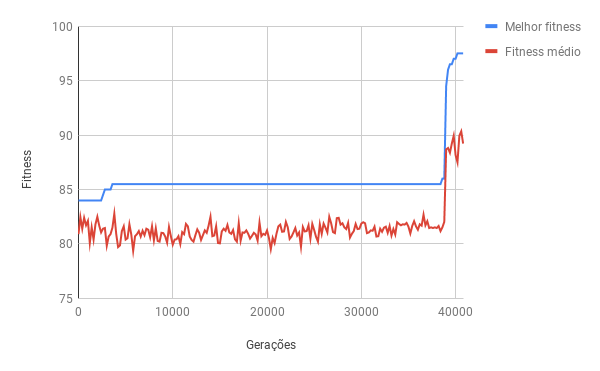
\includegraphics[scale=0.8]{images/resultado_97}
    \fautor
\end{figure}

Outro conjunto 2 de estados obteve uma resposta com taxa de acerto de 79 de 100 e 86,5 pontos. Nesse caso, o indivíduo com melhor resposta possui 4 genes, 2 genes destinas a resposta 0 e as demais respostas com apenas 1 gene. Apesar desse conjunto ter uma resposta muito inferior ao conjunto 1, ainda assim, o algoritmo evolutivo foi melhor do que uma tentativa de genes aleatórios, que obtiveram 77 acertos com 84 pontos. Ambos os resultados foram obtidos com aproximadamente 70.000 gerações. A Figura \ref{figura:resultado_79} mostra a evolução da função \fitness.

\begin{figure}[htb]
    \caption{Histórico de \fitness do conjunto 2 de estados.}
    \label{figura:resultado_79}
    \centering
    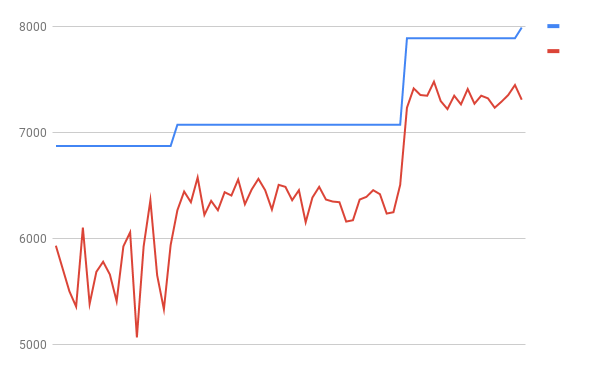
\includegraphics[scale=0.8]{images/resultado_79}
    \fautor
\end{figure}

Outros 10 conjuntos de estados foram analisados, a Figura \ref{figura:dez_execucoes} há resultados de execuções do algoritmo após 100.000 gerações, comparando o melhor indivíduo obtido pelo algoritmo com o melhor indivíduo obtido aleatoriamente, a figura mostra que o algoritmo obteve uma pontuação melhor do que tentativas aleatórias de acerto em todos os casos, evidenciando que o algoritmo caminha de alguma forma para uma solução.

\begin{figure}[htb]
    \caption{Resultado de dez execuções do algoritmo com 100.000 gerações comparando o melhor indivíduo obtido pela lógica da biblioteca com outro obtido aleatoriamente}
    \label{figura:dez_execucoes}
    \centering
    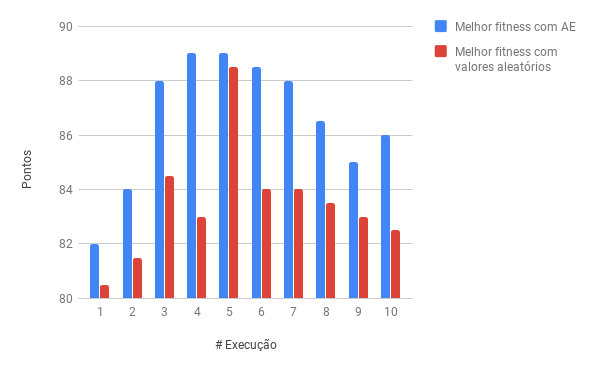
\includegraphics[scale=0.8]{images/dez_execucoes}
    \fautor
\end{figure}

\section{Dificuldades e Limitações}

\subsection{Sobre a biblioteca desenvolvida}

A biblioteca está implementada nos moldes citados e testada, entretanto, limita o usuário a linguagem Java. Idealmente a biblioteca deveria ser escrita em C/C++, compilada como executável de biblioteca dinâmica e adaptada para as mais diversas linguagens do mercado, essas mudanças ajudariam no desempenho e no reuso da biblioteca para outras linguagens. O projeto não foi desenvolvido dessa maneira pelas vantagens citadas na seção \ref{secao:rev_bib}, por se tratar de um material de estudo, os benefícios de Java foram importantes para o projetista.

\subsection{Sobre o algoritmo evolutivo para previsão de estados}

Os testes aplicados a esse estudos obtiveram resultados melhores do que vetores aleatórios, mas se demonstraram dependentes dos valores fornecidos. Em situações com uma amostragem de dados muito grande, é possível selecionar os melhores dados para alimentar o algoritmo evolutivo a fim de se encontrar os melhores parâmetros para previsão.

Os testes realizados foram com poucas entradas e com poucas saídas definidas, devido ao tempo computacional requerido para muitas entradas ou muitas saídas. Esse tema será discutido na seção de trabalhos futuros.

Embora os Algoritmos Evolutivos tenham sido exaustivamente explorados no meio acadêmico, os mesmos encontram resistência para serem aceitos no desenvolvimento de certas aplicações como jogos, devido ao fato de pesquisadores apontarem a técnica como lenta e capaz de permitir a obtenção de desempenhos ruins \cite{Sweetser2002} \cite{Spronck2003} \cite{Marcio2008}. Neste trabalho, os resultados não foram surpreendentes, são dependentes das entradas e análises com muitas entradas provocam lentidão.

\chapter{Conclusão}
\label{chapter:conclusao}
O algoritmo desenvolvido pode ser aplicado para diversas áreas da computação bio-inspirada e acrescenta um novo conceito sobre funções \fitness. A função \fitness pode ser obtida em casos de disputa entre dois jogadores comparando o desempenho entre eles numa disputa.

\chapter{Instalando o abnTeX2}
\label{chapter:instalando-abntex}

A instalação do \emph{abnTeX2} varia de acordo com o sistema operacional empregado pelo usuário. Aqui serão apresentadas as formas de instalação nos sistemas mais utilizados atualmente no curso de ciência da computação do Câmpus Catalão, a saber: Linux (Ubuntu 12.04), Mac OS X e Windows 7

\section{Linux (Ubuntu 12.04)}

Se você já instalou o Tex Live via apt-get, basta seguir os seguintes comandos:

\begin{enumerate}

\item Baixe os arquivos de instalação do abnTeX2 (\url{http://code.google.com/p/abntex2/downloads/list}). Nesse link você também encontra a documentação e exemplos de uso.
\item Extraia o conteúdo do arquivo baixado na pasta texmf local, geralmente /usr/local/share/texmf. 
\item Em um Terminal: extraia o ZIP: \emph{unzip abntex2.tds.zip} em qualquer local;
\item copie o conteúdo extraído para o destino: \emph{cp abntex2/* /usr/local/share/texmf};
\item Em um Terminal digite: \emph{sudo texhash}
\item Pronto!
\end{enumerate}

\section{Mac OS}

Primeiramente, deve-se abrir o terminal do Mac que pode ser encontrado em Aplicativos/Utilitários - buscando pelo Finder.  E seguir os comandos abaixo:
\begin{enumerate}
\item Baixe os arquivos de instalação do abnTeX2 (\url{http://code.google.com/p/abntex2/downloads/list}). Nesse link você também encontra a documentação e exemplos de uso.
\item Extraia o conteúdo do arquivo baixado na pasta \emph{texmf} local, geralmente \emph{/usr/local/texlive/texmf-local}
\item Em um Terminal digite: \emph{sudo texhash}
\item Pronto!
\end{enumerate}
 
 \section{Windows 7}

\subsection{Instalar/atualizar pelo Package Manager (recomendado)}

Geralmente o abnTeX2 é baixado e instalado automaticamente pelo MiKTeX quando o usuário compila pela primeira vez um dos modelos do abnTeX2. Porém, caso isso não ocorra, siga os passos seguintes:

\begin{enumerate}
\item Clique em Iniciar/Start -> Todos os Programas/All Programs -> MiKTeX -> Package Manager;
\item Clique em Repository / Synchronize;
\item Clique com o botão direito sobre \emph{abntex2} na lista e selecione Install (ou Update, caso já esteja instalado);
\item Pronto!
\end{enumerate}

\subsection{Instalar/atualizar manualmente}

Você apenas precisará utilizar a instalação manual no caso de:

\begin{enumerate}
\item o abnTeX2 não estar na lista de pacotes do MiKTeX por alguma razão;
\item você não poder utilizar uma conexão com a Internet no momento da instalação;
\item a versão do abnTeX2 no MiKTeX estar desatualizada em relação à versão disponível no CTAN.
\end{enumerate}
Em qualquer caso, lembre-se de remover uma eventual instalação anterior do abnTeX2 . Se houver instalado pelo Package Manager, remova o abnTeX2 também por ele.

Passos para instalação manual do abnTeX2 no MiKTeX:

\begin{enumerate}
\item Baixe os arquivos de instalação do abnTeX2 (abntex2.tds-vX.X.zip). Nesse link você também encontra a documentação e exemplos de uso.
\item Extraia o conteúdo do arquivo baixado em uma pasta qualquer;
\item Você pode criar uma pasta abntex2, por exemplo, em $C:\backslash abntex2\backslash$;
\item Consulte http://www.tex.ac.uk/cgi-bin/texfaq2html?label=install-where para outras informações;
\item Clique em Iniciar/Start -> Todos os Programas/All Programs -> MiKTeX -> Settings;
\item Na aba Roots, adicione o diretório recém criado;
\item Na aba General, clique em Refresh FNDB, OU, se preferir, em um Terminal digite initexmf --update-fndb;
\item Pronto!
\end{enumerate}

\chapter{Orientações Gerais}
\label{chapter:orientacoes-gerais}


\section{Codificação dos arquivos: UTF8}

A codificação de todos os arquivos do \abnTeX\ é \texttt{UTF8}. É necessário que
você utilize a mesma codificação nos documentos que escrever, inclusive nos
arquivos de base bibliográficas |.bib|.



\section{Inclusão de outros arquivos}\label{sec-include}

É uma boa prática dividir o seu documento em diversos arquivos, e não
apenas escrever tudo em um único. Esse recurso foi utilizado neste
documento. Para incluir diferentes arquivos em um arquivo principal,
de modo que cada arquivo incluído fique em uma página diferente, utilize o
comando:

\begin{verbatim}
   \include{documento-a-ser-incluido}      % sem a extensão .tex
\end{verbatim}

Para incluir documentos sem quebra de páginas, utilize:

\begin{verbatim}
   \input{documento-a-ser-incluido}      % sem a extensão .tex
\end{verbatim}



%\section{Remissões internas}

%Ao nomear a \autoref{tab-nivinv} e a \autoref{fig_circulo}, apresentamos um exemplo de remissão interna, que também pode ser feita quando indicamos o \autoref{cap_exemplos}, que tem o nome \emph{\nameref{cap_exemplos}}. O número do capítulo indicado é \ref{cap_exemplos}, que se inicia à \autopageref{cap_exemplos}\footnote{O número da página de uma remissão pode ser obtida também assim: \pageref{cap_exemplos}.}.
%Veja a \autoref{sec-divisoes} para outros exemplos de remissões internas entre seções, subseções e subsubseções.

%O código usado para produzir o texto desta seção é:

%\begin{verbatim}
%Ao nomear a \autoref{tab-nivinv} e a \autoref{fig_circulo}, apresentamos um
%exemplo de remissão interna, que também pode ser feita quando indicamos o
%\autoref{cap_exemplos}, que tem o nome \emph{\nameref{cap_exemplos}}. 
%O número
%do capítulo indicado é \ref{cap_exemplos}, que se inicia à
%\autopageref{cap_exemplos}\footnote{O número da página de uma remissão pode ser
%obtida também assim:
%\pageref{cap_exemplos}.}.
%Veja a \autoref{sec-divisoes} para outros exemplos de remissões internas entre
%seções, subseções e subsubseções.
%\end{verbatim}



\section{Consulte o manual da classe \textsf{abntex2}}

Consulte o manual da classe \textsf{abntex2} \cite{abntex2classe} para uma
referência completa das macros e ambientes disponíveis. 

Além disso, o manual possui informações adicionais sobre as normas ABNT
observadas pelo \abnTeX\ e considerações sobre eventuais requisitos específicos
não atendidos, como o caso da \citeonline[seção 5.2.2]{NBR14724:2011}, que
especifica o espaçamento entre os capítulos e o início do texto, regra
propositalmente não atendida pelo presente modelo.



\section{Precisa de ajuda?}

Consulte a FAQ com perguntas frequentes e comuns no portal do \abnTeX:
\url{https://code.google.com/p/abntex2/wiki/FAQ}.

Inscreva-se no grupo de usuários \LaTeX:
\url{http://groups.google.com/group/latex-br}, tire suas dúvidas e ajude
outros usuários.

Participe também do grupo de desenvolvedores do \abnTeX:
\url{http://groups.google.com/group/abntex2} e faça sua contribuição à
ferramenta.



\section{Você pode ajudar?}

Sua contribuição é muito importante! Você pode ajudar na divulgação, no
desenvolvimento e de várias outras formas. Veja como contribuir com o \abnTeX\
em \url{https://code.google.com/p/abntex2/wiki/ComoContribuir}.

\chapter{Configuração dos Elementos Pré-Textuais}
\label{chapter:config-pre-textual}
A configuração de diversas opções e principalmente dos elementos pré-textuais é realizada com comandos específicos inseridos antes do comando \comando{begin\{document\}}. As informações do documento são configuradas através dos comandos:

\begin{description}

 \item[\comando{titulo\{T\}}] Título do trabalho (substitua T pelo título do trabalho);

 \item[\comando{autor[REF]\{N\}}] Nome do autor do trabalho (onde REF é como o nome do autor é referenciado e N é o nome do autor);

 \item[\comando{orientador\{T\}\{O\}}] Nome do professor orientador do trabalho. Caso seja uma orientadora pode ser usado o comando \comando{orientador[Orientadora:]\{T\}\{O\}} (sendo que T é a titulação do professor e O é o nome do orientador);

 \item[\comando{coorientador\{T\}\{C\}}] Nome do professor coorientador do trabalho. Caso seja uma coorientadora pode ser usado um comando análogo a definição de orientadora  empregando o comando \comando{coorientador[Coorientadora:]\{T\}\{C\}}(sendo que T é a titulação do professor e C é o nome do orientador);

 
 \item[\comando{curso\{EP\}\{NP\}}] Dados do programa de Pós-Graduação (onde EP é a especialidade que será atribuída ao pós-graduando e NP é o nome do programa de pós-graduação.  Exemplo: \comando{curso\{Ciências -- Ciências de Computação e Matemática Computacional\}\{Ciências de Computação e Matemática Computacional\}};
 
 \item[\comando{data\{dia\}\{mês\}\{ano\}}] Configuração da data do depósito do documento;

 \item[\comando{textoresumo\{TR\}\{PC\}}] Texto do resumo (TR) e palavras-chave (PC) do documento sendo separadas por vírgula. Se o idioma do resumo for diferente do declarado no documento, pode ser usado o comando \comando{textoresumo[L]\{TR\}\{PC\}} (sendo que L é a linguagem do resumo).
 
\end{description}

As opções seguintes correspondem também as configurações dos elementos pré-textuais, porém seu uso é opcional: 

\begin{description}

 \item[\comando{textodedicatoria\{TD\}}] Texto referente a dedicatória do trabalho (TD). Caso o texto esteja em um arquivo separado (recomendado para que o projeto fique modularizado e os documentos mais limpo), deve utilizar o comando \comando{textodedicatoria*\{ARQ\}}, em que ARQ é o nome do arquivo, incluindo o caminho do diretório se necessário;

 \item[\comando{textoagradecimentos\{TA\}}] Texto referente aos agradecimentos do trabalho (TA). Caso o texto esteja em um arquivo separado (recomendado para que o projeto fique modularizado e os documentos mais limpo), deve utilizar o comando \comando{textoagradecimentos*\{ARQ\}}, em que ARQ é o nome do arquivo, incluindo o caminho do diretório se necessário;

 \item[\comando{incluilistadefiguras}] Comando para inclusão da lista de figuras. Deve-se utilizar este comando somente quando o ambiente \textbf{figure} for utilizado no documento;
 
 \item[\comando{incluilistadetabelas}] Comando para inclusão da lista de tabelas. Deve-se utilizar este comando somente quando o ambiente \textbf{table} for utilizado no documento;
  
 \item[\comando{incluilistadequadros}] Comando para inclusão da lista de quadros. Deve-se utilizar este comando somente quando o ambiente \textbf{quadro} for utilizado no documento;
   
 \item[\comando{incluilistadealgoritmos}] Comando para inclusão da lista de algoritmos. Deve-se utilizar este comando somente quando o ambiente \textbf{algoritmo} for utilizado no documento;
    
 \item[\comando{incluilistadecodigos}] Comando para inclusão da lista de figuras. Deve-se utilizar este comando somente quando o ambiente \textbf{codigo} for utilizado no documento;
 
 \item[\comando{incluilistadesiglas}] Comando para inclusão da lista de siglas e abreviaturas. Deve-se utilizar este comando somente quando existirem siglas e abreviaturas no documento, com a utilização do comando \comando{sigla\{S\}\{DS\}} ou \comando{sigla*\{S\}\{DS\}};

 \item[\comando{incluilistadesimbolos}] Comando para inclusão da lista de símbolos. Deve-se utilizar este comando somente quando existirem símbolos no documento, com a utilização do comando \comando{simbolo\{S\}\{DS\}}.
 
\end{description}

\chapter{Corpos Flutuantes}
\label{chapter:corpos-flutuantes}

Corpos flutuantes são elementos não textuais, como figuras e tabelas, que complementam as informações do texto. Neste capítulo são expostos breves exemplos dos corpos flutuantes disponíveis na classe \textit{icmc}.

Na \autoref{secao:figuras} é mostrado como inserir figuras, a \autoref{secao:tabelas_e_quadros} explica como incluir tabelas e quadros, a \autoref{secao:algoritmos_e_codigos} demostra como trabalhar com algoritmos e códigos-fonte e a \autoref{secao:outros-ambientes} explica como definir outros ambientes para serem utilizados, como para gráficos e diagramas.

\section{Figuras}
\label{secao:figuras}

A inserção de figuras é realizada normalmente através do comando \comando{begin\{figure\}}. Na \autoref{figura:logomarca_usp} é exibida a logomarca da USP com o pacote \textit{graphicx}. Já a \autoref{figura:exemplo_grafo} mostra um exemplo de grafo com o pacote \textit{xy}. De acordo com as normas ABNT a lista de figuras é um elemento opcional do documento, para incluí-la é preciso inserir o comando \comando{incluidelistafiguras} antes do início do documento.

Observe que, segundo a \citeonline[seções 4.2.1.10 e 5.8]{NBR14724:2011}, as
ilustrações devem sempre ter numeração contínua e única em todo o documento. Além disso, deve ser incorporado ao corpo flutuante do tipo figura, além da legenda, a fonte de onde esta foi extraída. Se a figura foi confeccionada pelo próprio autor, deve se colocar "Elaborada pelo autor".

\begin{citacao}
Qualquer que seja o tipo de ilustração, sua identificação aparece na parte
superior, precedida da palavra designativa (desenho, esquema, fluxograma,
fotografia, gráfico, mapa, organograma, planta, quadro, retrato, figura,
imagem, entre outros), seguida de seu número de ordem de ocorrência no texto,
em algarismos arábicos, travessão e do respectivo título. Após a ilustração, na
parte inferior, indicar a fonte consultada (elemento obrigatório, mesmo que
seja produção do próprio autor), legenda, notas e outras informações
necessárias à sua compreensão (se houver). A ilustração deve ser citada no
texto e inserida o mais próximo possível do trecho a que se
refere. \cite[seções 5.8]{NBR14724:2011}
\end{citacao}

\begin{figure}[htb]
 \caption{Logomarca da USP}
 \label{figura:logomarca_usp}
 \centering
 
\includegraphics[scale=0.3]{images/usp-logo}
 \fdireta{usp:logo}
\end{figure}


\begin{figure}[htb]
\caption{Exemplo de grafo}
\label{figura:exemplo_grafo}
\centering
\begin{scriptsize}
$$
\xymatrix@R20pt@C10pt{
 & & & & vr \ar[dlll] \ar[dl] \ar[d] \ar[dr] \ar[drr] \ar[drrr] & & & \\
 & (a_3, b_2, c_1) \ar[d]^{\varphi_2} \ar[dl]_{\varphi_1} & & (a_3, b_2, c_2) \ar[d]^{\varphi_2} \ar[dl]_{\varphi_1} & (a_1, b_1, c_1) & (a_1, b_1, c_2) & (a_1, b_2, c_1) & (a_1, b_2, c_2) \\
 (a_2, b_2, c_1) \ar[dr]_{\varphi_3} & (a_3, b_1, c_1) \ar[d]^{\varphi_1} & (a_2, b_2, c_2) \ar[dr]_{\varphi_3} & (a_3, b_1, c_2) \ar[d]^{\varphi_1} & & & & \\
& (a_2, b_1, c_1)  & & (a_2, b_1, c_2) & & & & \\
}
$$
\end{scriptsize}
\fautor
\end{figure}

A classe \textit{icmc} traz algum comando que auxiliam na inserção da legenda, para utilizá-los basta substituir o \comando{fonte\{\}} por um dos seguintes comando conforme necessário:

\begin{description}

 \item[\comando{fautor}] Insere o texto \aspas{Elaborada pelo autor} como fonte da figura;

 \item[\comando{fadaptada[INF]\{REF\}}] Insere um texto informando que a figura foi adaptada de alguma referência bibliográfica (REF). INF refere-se ao local específico de onde a imagem foi extraída, como por exemplo o número da página. Além disso, INF é um parâmetro opcional e pode receber qualquer cadeia de texto;

 \item[\comando{fdireta[INF]\{REF\}}] Insere um texto informando que a figura próvem diretamente de alguma referência bibliográfica (REF). INF refere-se ao local específico de onde a imagem foi extraída, como por exemplo o número da página. Além disso, INF é um parâmetro opcional e pode receber qualquer cadeia de texto;
 
 \item[\comando{fdadospesquisa}] Insere o texto \aspas{Dados da pesquisa.} como fonte da figura;
 
\end{description}



\section{Tabelas e Quadros}
\label{secao:tabelas_e_quadros}

A inserção de tabelas e quadros é feita de forma semelhante a inserção de figuras, porém são utilizados os ambientes \textit{table} e \textit{quadro}. A principal diferença entre tabelas e quadros, de acordo com \citeonline{silveira:2006:manual_tcc}, é que as tabelas são destinadas para informações numéricas e os quadros são mais adequados para informações textuais. Em geral, as tabelas devem estar padronizadas conforme o padrão do
\citeonline{ibge1993} requerido pelas normas da ABNT para documentos técnicos e
acadêmicos.

Como exemplos foram inseridas a \autoref{tabela:lista_produtos} que exibe uma de lista de produtos (construída em \LaTeX) e a Tabela \autoref{tabela:populacao_america_sul} que mostra a população dos países da América do Sul (construída segundo o padrão do IBGE). Foi inserido também o \autoref{quadro:editores_texto_livres} com alguns editores que podem ser usados para se trabalhar com \LaTeX para demonstrar a inserção de quadros.

 A lista de tabelas também é um elemento opcional que pode ser incluída com o comando \comando{incluidelistatabelas} antes do início do documento. O mesmo acontece com a lista de quadros que pode ser incluída com o comando \comando{incluidelistaquadros}.

\begin{table}[htb]
\centering
\caption{Lista de produtos}
\label{tabela:lista_produtos}
\begin{tabularx}{\textwidth}{X|l|r|r|r} \hline
Produto      & Unidade & Preço (R\$) & Quantidade & Total (R\$) \\ \hline
Arroz        & Kg      & 2,00        & 550        & 1.100,00    \\
Óleo de Soja & L       & 2,50        & 500        & 750,00      \\
Açucar       & Kg      & 3,00        & 100        & 300,00      \\ \hline
\end{tabularx}
\fdadospesquisa
\end{table}

\begin{table}[htb]
\IBGEtab{%
  \caption{População dos países da América do Sul} \label{tabela:populacao_america_sul}
}{%
\begin{tabular}{r|p{3cm}|r}        
\toprule
Código  & País            & População   \\ \midrule \midrule
1       & Brasil          & ~~~~~~191.480.630 \\ \midrule 
2       & Argentina       &  39.934.100 \\ \midrule 
3       & Colômbia        &  46.741.100 \\ \midrule 
4       & Paraguai        &   9.694.200 \\ \midrule 
5       & Uruguai         &   3.350.500 \\ \midrule 
6       & Peru            &  28.221.500 \\ \midrule 
7       & Equador         &  13.481.200 \\ \midrule 
8       & Bolívia         &   9.694.200 \\ \midrule 
9       & Venezuela       &  28.121.700 \\ \midrule 
10      & Chile           &  16.803.000 \\ \bottomrule
\end{tabular}
}{%
  \fdireta{wikipedia:2011:america_sul}%
  \nota{Esta é uma nota, que diz que os dados são baseados na
  regressão linear.}%
  \nota[Anotações]{Uma anotação adicional, que pode ser seguida de várias
  outras, porém são opcionais.}%
  }
\end{table}

\begin{quadro}[htb]
\caption{Editores de Texto Livres}
\label{quadro:editores_texto_livres}
\centering
\begin{tabular}{|l|l|r|}        \hline
Editor     & Multiplataforma & Específico para Latex \\ \hline
Kwriter    & Sim             & Não                   \\
Texmaker   & Sim             & Sim                   \\
Kile       & Sim             & Sim                   \\
Geany      & Sim             & Não                   \\ \hline
\end{tabular}
\end{quadro}

\section{Algoritmos e Códigos}
\label{secao:algoritmos_e_codigos}

Além dos corpos flutuantes convencionais para inserir figuras (\comando{begin\{figure\}}) e tabelas (\comando{begin\{table\}}), a classe \textit{icmc} possui mais dois tipos de corpos flutuantes um para algoritmos (\comando{begin\{algoritmo\}}) e outro para códigos-fonte (\comando{begin\{codigo\}}). A utilização de um ou de outro fica a critério do usuário. Como exemplo temos o \autoref{algoritmo:mdc1} que calcula o máximo divisor comum entre dois números e os Códigos-fonte \ref{codigo:notas_alunos} e \ref{codigo:metodo_leitura} que são uma consulta na \sigla{SQL}{\textit{Structured Query Language}} e uma sobrotina em \textit{Java}.

%\begin{algoritmo}[htb]
\begin{algoritmo}
%\begin{algorithmic}[1]
\caption{Algoritmo para cálculo de máximo divisor comum MDC($n_1$,$n_2$)}
\label{algoritmo:mdc1}

 \KwIn{Dois números inteiros ($n_1, n_2$)}
 \If(\tcp*[f]{Garante que o maior número seja $n_1$}){$n_2 > n_1$}
   {troca valores de $n_1$ e $n_2$}
 \Repeat{$r > 0$}{
    $r \leftarrow$ resto da divisão de $n_1$ por $n_2$
    $n_1 \leftarrow n_2$
    $n_2 \leftarrow r$
 }
 \Return $n_1$
%\end{algorithmic}
\end{algoritmo}
%\end{algoritmo}

%\begin{codigo}[htb]
%\caption{Consulta SQL}
%\label{codigo:notas_alunos}
%\hrule
\begin{codigo}[caption = {Consulta SQL}, label={codigo:notas_alunos},language=SQL, breaklines=true]
SELECT a.nome_aluno AS aluno,
       d.nome_disciplina AS disciplina,
       m.nota AS nota
FROM aluno AS a,
     disciplina AS d,
     matriculado AS m
WHERE a.id_aluno = m.id_aluno
  AND d.id_disciplina = m.id_disciplina
ORDER BY a.nome_aluno, d.nome_disciplina;
\end{codigo}
%\end{codigo}

%\begin{codigo}[htb]
%\caption{Subrotina para obter uma entrada do usuário}
%\label{codigo:metodo_leitura}
%\hrule
\begin{codigo}[caption={Subrotina para obter uma entrada do usuário}, label={codigo:metodo_leitura}, language=Java, breaklines=true]
public static String Leitura(){
    BufferedReader reader = new BufferedReader(new InputStreamReader(System.in));
    try {
        return reader.readLine(); // Lê uma linha pelo teclado
    } catch (IOException e) {
        e.printStackTrace();
        return "";
    }
}
\end{codigo}
%\end{codigo}

Existem diversos outros pacotes disponíveis para escrever algoritmos e códigos. Nos exemplos anteriormente foram utilizados o pacote \textit{algorithm} para definição do ambiente algoritmo e \textit{listings} para a definição do ambiente de código-fonte. O pacote \textit{algorithm} é usado para escrever algoritmos em alto nível \cite{janos:2005:algpseudocode}. Já o pacote \textit{listings} serve para escrever os códigos em diversas linguagens de programação \cite{moses:2006:listings}.

Caso sejam utilizados os ambientes de algoritmos e código podem ser incluídos os comandos \comando{incluidelistaalgoritmos} e \comando{incluidelistacodigos} antes do \comando{begin\{document\}} para que a lista de algoritmos e a lista de código sejam criadas.


\section{Ambientes Matemáticos}

A classe \textit{icmc} provê os seguintes ambientes matemáticos:
\begin{itemize}
 \item Teoremas (\comando{begin\{teorema\}[\ ]} ... \comando{begin\{teorema\}});
 \item Proposição (\comando{begin\{proposicao\}[\ ]} ... \comando{begin\{proposicao\}});
 \item Lema (\comando{begin\{lema\}[\ ]} ... \comando{begin\{lema\}});
 \item Corolário (\comando{begin\{corolario\}[\ ]} ... \comando{begin\{corolario\}});
 \item Exemplo (\comando{begin\{exemplo\}[\ ]} ... \comando{begin\{exemplo\}});
 \item Observação (\comando{begin\{observacao\}[\ ]} ... \comando{begin\{observacao\}});
 \item Definição (\comando{begin\{definicao\}[\ ]} ... \comando{begin\{definicao\}});
 \item demonstracao (\comando{begin\{demonstracao\}[\ ]} ... \comando{begin\{demonstracao\}}).
\end{itemize}

Abaixo temos um exemplo de proposição com sua demonstração:
\begin{proposicao}
 Sejam $a$ e $b$ reais, tais que $0<a<b$. Então $a^2<b^2$.
\end{proposicao}
\begin{demonstracao}
 Pela hipótese concluímos que $(b+a)>0$ e $(b-a)>0$.

Como $b^2-a^2=(b+a)(b-a)$ concluímos que $b^2-a^2>0$, ou seja, $a^2<b^2$.
\end{demonstracao}

Neste documento tratamos brevemente apenas dos ambientes mencionados anteriormente. Contudo, para escrever expressões matemáticas complexas é preciso estudar uma documentação mais específica como em \citeonline{cassagojr:1997:amslatex}.

Alguns dos ambientes matemáticos da classe \textit{icmc} podem ser usados também para outras finalidades como exemplos e definições.


\section{Definição de outros ambientes}
\label{secao:outros-ambientes}

O classe \textit{icmc} permite a criação de outros ambientes, além dos citados nas seções anteriores, caso seja necessário. Isso é possível graças a extensão da classe \textit{abntex}. O \autoref{codigo:novo-ambiente} deve ser inserido antes do início do documento para criação de um ambiente para gráficos. Para definição de outros ambientes, basta seguir o modelo.


\begin{codigo}[caption={Definição do ambiente \textbf{grafico}}, label={codigo:novo-ambiente}, language=Tex, breaklines=true]
\makeatletter

% Novo list of (listings) para GRÁFICOS --------------------------
\newcommand{\graficoname}{Gráfico}
\newcommand{\graficorefname}{Gráfico}
\newcommand{\listofgraficosname}{Lista de gráficos}

\addto\captionsenglish{% ingles
    %% adjusts names from abnTeX2
    \newcommand{\graficoname}{Graph}
    \newcommand{\graficorefname}{Graph}
    \newcommand{\listofgraficosname}{List of graphs}
}

\newfloat[chapter]{grafico}{logr}{\graficoname}
\newlistof{listofgraficos}{logr}{\listgraficoname}
\newlistentry{grafico}{logr}{0}

% configurações para atender às regras da ABNT
\renewcommand{\thegrafico}{\thechapter.\@arabic\c@grafico}
\setfloatadjustment{grafico}{\centering}
\renewcommand{\cftgraficoname}{\graficoname\space}
\renewcommand*{\cftgraficoaftersnum}{\hfill\textendash\hfill}
% ----------------------------------------------------------------

\makeatother
\end{codigo}

A utilização do novo ambiente no texto segue conforme o \autoref{codigo:usar-novo-ambiente}.

\begin{codigo}[caption={Como usar o ambiente \textbf{grafico}}, label={codigo:usar-novo-ambiente}, language=Tex, breaklines=true]
\begin{grafico}[htb]
\caption{Caption do gráfico}
\label{gra:modelo}
Este é o conteúdo do gráfico.
\end{grafico}
\end{codigo}

Comandos como \comando{autoref\{gra:modelo\}} funcionam normalmente.

Para imprimir a "Lista de gráficos" no documento, insira o \autoref{codigo:lista-novo-ambiente} na classe \textit{icmc}, de modo que ele seja impresso após a "Lista de ilustrações". O código deve ser inserido após a linha 1244.


\begin{codigo}[caption={Código para inserir lista de gráficos}, label={codigo:lista-novo-ambiente}, language=Tex, breaklines=true]
% ---
% inserir lista de gráficos
% ---
\pdfbookmark[0]{\listofgraficosname}{logr}
\listofgraficos*
\cleardoublepage
% ---
\end{codigo}

\chapter{Listas}
\label{chapter:listas}
\section{Abreviaturas e Siglas}

A classe \textit{icmc} implementa a criação da lista de abreviaturas e siglas com o pacote \textit{nomencl}. A inserção de abreviaturas e siglas na lista é realizada com o comando \comando{sigla\{A\}\{B\}}, onde \textit{A} é a sigla e \textit{B} é o nome por extenso. Para se gerar a lista de siglas na parte pre-textual é preciso incluir o comando \comando{incluidelistasiglas} antes do início do documento. Além disto, a compilação do documento deve conter o comando \textit{makeindex} após duas compilações com o \textit{pdflatex}. Por exemplo, supondo que o documento principal tenha o nome de \textit{monografia}, podemos usar a seguinte sequência de comandos:
\begin{verbatim}
pdflatex monografia.tex
pdflatex monografia.tex
makeindex monografia.nlo -s nomencl.ist -o monografia.nls
pdflatex monografia.tex
\end{verbatim}

No Capítulo \ref{chapter:ferramentas-uteis} serão apresentadas algumas ferramentas que podem facilitar o processo de compilação do documento.

\section{Símbolos}

A definição de símbolos é semelhante a definição de siglas, porém deve ser usado o comando \comando{simbolo\{S\}\{DS\}}, onde \textit{S} é o símbolo e \textit{DS} é a descrição do símbolo. Como exemplo definimos os símbolos \simbolo{\mathbb{X}}{Variável X}$\mathbb{X}$ e \simbolo{\mathsf{I\!R}}{Conjunto dos números reais}$\mathsf{I\!R}$. Para incluir a lista de símbolos, basta usar o comando \comando{incluidelistasimbolos} antes do início do documento.


\chapter{Ferramentas Úteis}
\label{chapter:ferramentas-uteis}
Existem diversas ferramentas para se trabalhar com \LaTeX. Duas ferramentas que merecem destaque são o editor \textit{Texmaker} exibido na Figura \ref{figura:texmaker} e o gerenciador de referências \textit{JabRef} mostrado na Figura \ref{figura:jabref}. Ambas ferramentas são livres e multiplataforma.

\begin{figure}[htb]
\caption{Tela do Texmaker}
 \label{figura:texmaker}
 \centering
 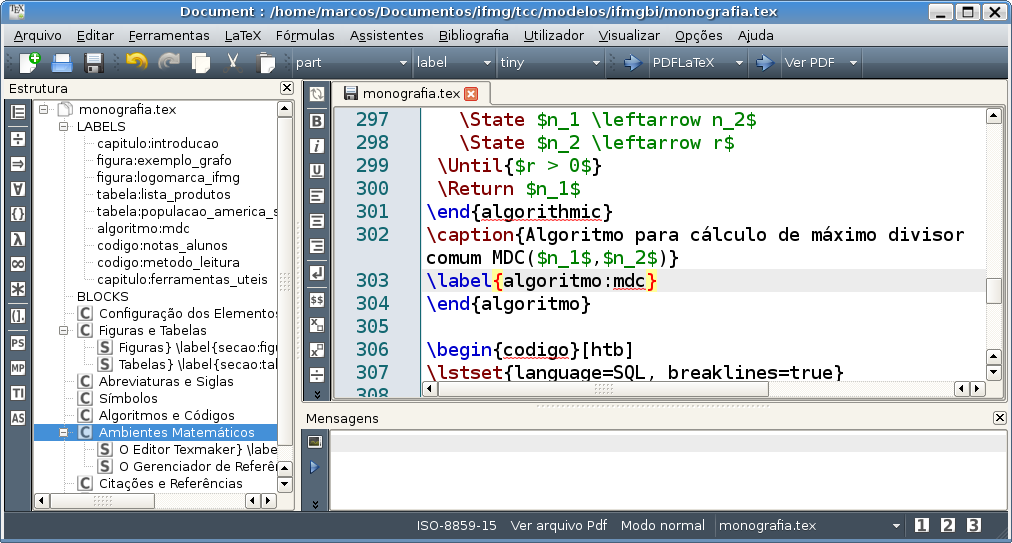
\includegraphics[width=\textwidth]{texmaker}
 \legend{Fonte: o autor.}
\end{figure}

\begin{figure}[htb]
 \caption{Tela do JabRef}
 \label{figura:jabref}
 \centering
 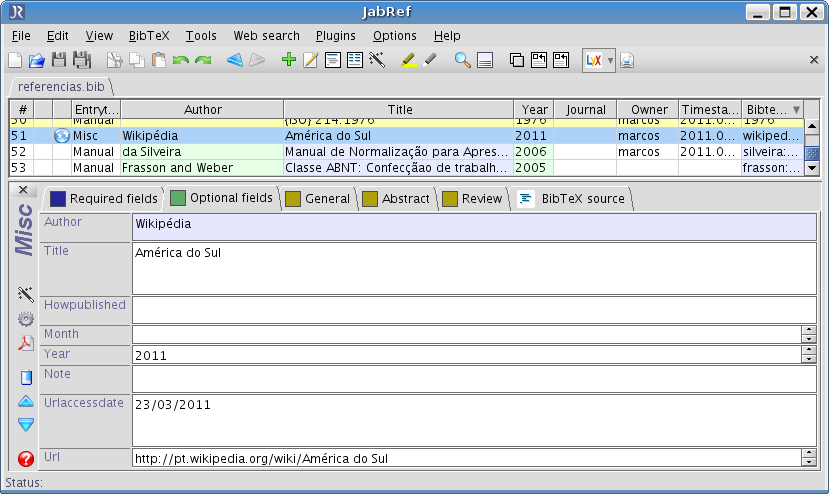
\includegraphics[width=\textwidth]{jabref}
\legend{Fonte: o autor.}
\end{figure}

O Texmaker pode ser obitido em \url{www.xm1math.net/texmaker} e o JabRef pode ser obtido em \url{jabref.sourceforge.ne}. É importante ressaltar que o Texmaker é apenas um editor, para compilar os documentos é necessário um ambiente \LaTeX instalado. Os ambientes Latex mais populares são o Texlive (\url{www.tug.org/texlive}) e o MiKTex (\url{miktex.org}).

\chapter{Citações e Referências}
\label{chapter:citacoes}
Em documentos acadêmicos podem existir citações diretas e citações indiretas. As citações indiretas são feitas quando se reescreve uma referência consultada. Nas citações indiretas há duas formatações possíveis dependendo de como ocorre a citação no texto. Quando o autor é mencionado explicitamente  deve ser usado o comando \comando{citeonline\{\}}, nas demais situações é usado o comando \comando{cite\{\}}. No quadro \ref{figura:citacao_indireta_explicita} encontrasse um  exemplo de uso do comando \comando{citeonline\{\}}.

\begin{quadro}[htb]
\caption{Exemplo de citação indireta explícita} \label{figura:citacao_indireta_explicita}
\hrulefill

\lstset{language=Tex, breaklines=true}
\begin{lstlisting}
Segundo \citeonline{silveira:2006}, o trabalho de conclusão de curso deve seguir as normas da ABNT.
\end{lstlisting}

\hrulefill

Segundo \citeonline{silveira:2006:manual_tcc}, o trabalho de conclusão de curso deve seguir as normas da ABNT.

\hrulefill

%\legend{Fonte: o autor.}
\end{quadro}

Para especificar a página consultada na referência é preciso acrescentá-la entre colchetes com os comandos \comando{cite[página]\{\}} ou \comando{citeonline[página]\{\}}. No quadro \ref{figura:citacao_indireta_pagina} é mostrado um exemplo de citação com página específica.

\begin{quadro}[htb]
\caption{Exemplo de citação indireta não explícita} \label{figura:citacao_indireta_pagina}
\hrulefill

\lstset{language=Tex, breaklines=true}
\begin{lstlisting}
A folha de aprovação é um elemento obrigatório na monografia de projeto final de curso trabalho de conclusão de curso.  \cite[p.~10]{silveira:2006}.
\end{lstlisting}

\hrulefill

A folha de aprovação é um elemento obrigatório no trabalho de conclusão de curso.  \cite[p.~10]{silveira:2006:manual_tcc}.

\hrulefill

\end{quadro}

As citações diretas acontecem quando o texto de uma referência é transcrito literalmente. As citações diretas são curtas (até três linhas) são inseridas no texto entre aspas duplas. Conforme exemplo no quadro \ref{figura:citacao_direta_curta}.

\begin{quadro}[htb]
\caption{Exemplo de citação direta curta}
\label{figura:citacao_direta_curta}
\hrulefill

\lstset{language=Tex, breaklines=true}
\begin{lstlisting}
``Os quadros, ao contrário das tabelas, apresentam dados textuais e devem localizar-se o mais próximo do texto a que se referem'' \cite[p.~25]{silveira:2006}.
\end{lstlisting}

\hrulefill

``Os quadros, ao contrário das tabelas, apresentam dados textuais e devem localizar-se o mais próximo do texto a que se referem'' \cite[p.~25]{silveira:2006:manual_tcc}.

\hrulefill
\end{quadro}

As citações longas (com mais de 3 linhas) podem ser inseridas via \comando{begin\{citacao\}} conforme quadro \ref{figura:citacao_direta_longa}.

\begin{quadro}[htb]
\caption{Exemplo de citação direta longa}
\label{figura:citacao_direta_longa}
\hrulefill

\lstset{language=Tex, breaklines=true}
\begin{lstlisting}
\begin{citacao}
Síntese final do trabalho, a conclusão constitui-se de uma resposta à hipótese enunciada na introdução. O autor manifestará seu ponto de vista sobre os resultados obtidos e sobre o alcance dos mesmos. Não se permite a inclusão de dados novos nesse capítulo nem citações ou interpretações de outros autores \cite[p.~25]{silveira:2006}.
\end{citacao}
\end{lstlisting}

\hrulefill

\begin{citacao}
Síntese final do trabalho, a conclusão constitui-se de uma resposta à hipótese enunciada na introdução. O autor manifestará seu ponto de vista sobre os resultados obtidos e sobre o alcance dos mesmos. Não se permite a inclusão de dados novos nesse capítulo nem citações ou interpretações de outros autores \cite[p.~25]{silveira:2006:manual_tcc}.
\end{citacao}

\hrulefill

\end{quadro}


% ---
% Finaliza a parte no bookmark do PDF, para que se inicie o bookmark na raiz
% ---
\bookmarksetup{startatroot}% 
% ---

% ----------------------------------------------------------
% ELEMENTOS PÓS-TEXTUAIS
% ----------------------------------------------------------
\postextual

% ----------------------------------------------------------
% Referências bibliográficas
% ----------------------------------------------------------
\bibliography{references}

% ---------------------------------------------------------------------
% GLOSSÁRIO
% ---------------------------------------------------------------------

% Arquivo que contém as definições que vão aparecer no glossário
\newword{30}{Função fitness}{Função que pode medir o quão boa é uma solução em uma escala numérica}

\newword{35}{Java}{Linguagem de programação orientada a objetos que gera um \textit{bytecode} para ser interpretado pela JVM, portanto, é uma linguagem semi-compilada, trazendo benefícios de linguagens compiladas e interpretadas}

\newword{36}{Java Virtual Machine}{JVM é uma máquina virtual que possibilita um computador executar programas em Java}


% Comando para incluir todas as definições do arquivo glossario.tex
\glsaddall
% Impressão do glossário
\printglossaries

% ----------------------------------------------------------
% Apêndices
% ----------------------------------------------------------

% ---
% Inicia os apêndices
% ---
\begin{apendicesenv}

    \chapter{Documento Básico Usando a Classe icmc}
    \label{chapter:documento-basico}
    
\begin{codigo}[caption={Exemplo de um documento básico}, label={codigo:documento-basico}, language=Tex, breaklines=true]
% Documento utilizando a classe ufgcac
% Opções: 
%   Qualificação         = qualificacao 
%   Curso                = doutorado/mestrado
%   Situação do trabalho = pre-defesa/pos-defesa (exceto para qualificação)
% -- opções do pacote babel --
% Idioma padrão = brazil
	%french,	    % idioma adicional para hifenização
	%spanish,			% idioma adicional para hifenização
	%english,			% idioma adicional para hifenização
	%brazil				% o último idioma é o principal do documento
\ documentclass[doutorado, spanish, english, brazil]{packages/icmc}

% Título do trabalho
\titulo{Título da Monografia}

% Nome do autor
\autor[Abreviação]{Nome completo do autor}

% Define o local
\local{São Carlos -- SP}

% Data do depósito
\data{18}{12}{2012}

% Nome do Orientador
\orientador[Orientador:]{Titulação do orientador}{Nome completo do Orientador}

% Nome do Coorientador (caso não exista basta remover)
\coorientador[Coorientador:]{Titulação do coorientador}{Nome completo do Coorientador}
% Se coorientadora troque Coorientador: por Coorientadora: dentro do colchetes

% Define o nome da instituição
\instituicao{Instituto de Ciências Matemáticas e de Computação (ICMC/USP)}

% Especiolidade e Nome do programa de Pós-graduação
\curso[Ciências -- Ciências de Computação e Matemática Computacional]{Ciências de Computação e Matemática Computacional}
% O valor entre colchetes é opcional

% Resumo
\textoresumo[Idioma]{
Texto do resumo do trabalho.
}{Lista de palavras-chave separada por virgulas}


% Início do documento
\begin{document}

\chapter{Introdução}

Capítulo de Introdução

\chapter{Desenvolvimento}

Capítulo de Desenvolvimento

\chapter{Conclusão}

Capítulo de conclusão

% Nome do arquivo com as referências bibliográficas
\bibliography{referencias}

\end{document}

\end{codigo}

\end{apendicesenv}
% ---


% ----------------------------------------------------------
% Anexos
% ----------------------------------------------------------

% ---
% Inicia os anexos
% ---
\begin{anexosenv}

    \chapter{Páginas Interessantes na Internet} 
    \label{chapter:paginas-interessantes}
    \begin{description}
 \item[\url{http://www.tex-br.org}]: Página em português com diversos tutoriais e referências interessantes sobre \LaTeX;
 \item[\url{http://en.wikibooks.org/wiki/LaTeX}]: Livro em formato \textit{wiki} gratuito sobre \LaTeX;
 \item[\url{http://tobi.oetiker.ch/lshort/lshort.pdf}]: Ótimo tutorial sobre \LaTeX (possui versão em português \url{http://alfarrabio.di.uminho.pt/~albie/lshort/ptlshort.pdf}, mas a versão em inglês é a mais atual);
 \item[\url{http://code.google.com/p/abntex2/}]: Página do abnTeX2, grupo que desenvolve os pacotes e classes em \LaTeX para as normas da ABNT, nos quais a classe \textit{icmc} foi baseada;
\item[\url{ http://www.rexlab.ufsc.br:8080/more/index.jsp}]: Página do Mecanismo On-line para Referências  (MORE) desenvolvido pela UFSC.
 \end{description}

\end{anexosenv}
% ---

\end{document}